\begin{exercise}
  Wir betrachten das zweidimensionale Poisson Problem mit homogenen
  Dirichlet-Randbedingungen, siehe $(7.19)$ des Vorlesungsskriptes. Geben Sie
  die Diskretisierungsmatrix $A_h$ und die rechte Seite $g_h$ des entstehenden
  linearen Gleichungssystems an, wenn dieses Problem mit Finiten Differenzen der
  Schrittweite $h_1 = h_2 = h > 0$ diskretisiert wird. Beginnen Sie der Einfachheit
  halber mit dem Gitter aus Abb. 1. Dazu sollten Sie die Unbekannten
  $y_{j,k} \approx y(x_{j,k})$ wie folgt ordnen

  \begin{align}\label{sec}
    y_{1,1}, \dots , y_{1,N_2 -1}, \text{ }
    y_{2,1}, \dots , y_{2,N_2 -1} \text{ }
    y_{3,1}, \dots
  \end{align}
  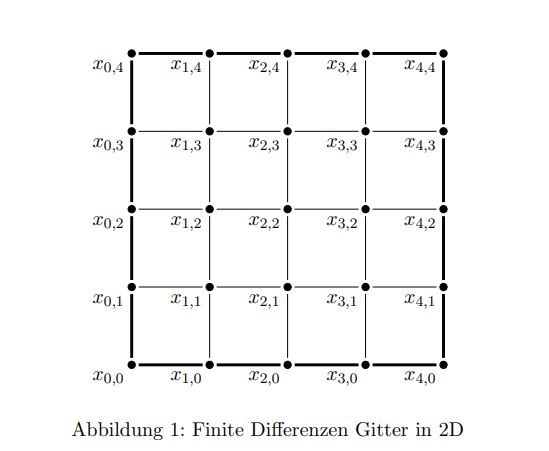
\includegraphics{Abbildung_1}
  \end{exercise}

\begin{solution}
  Im Skript haben wir die Gleichungen für das zweidimensionale Poisson Problem
  für $j = 1,\dots, N-1$ und $k = 1,\dots, N-1$ gegeben.

  \begin{align*}
    -\frac{1}{h^2}(y_{j-1,k} + y_{j+1,k}
    + y_{j,k-1} + y_{j,k+1}
    - 4 y_{j,k})
    =
    f(x_{j,k})
  \end{align*}

  Falls nun $j=0, j=N, k = 0$ oder $k=N$, also genau am Gitterrand,
  gilt wegen der Dirichlet-Randbedingungen $y_{j,k} = 0$.

  Unsere Unbekannten wie in der Angabe georndet und in einen Vektor verpackt:

  \begin{align*}
    y = (y_{11}, y_{12}, \dots, y_{1,N-1}, y_{21}, \dots, y_{N-1,N-1})^\top
  \end{align*}

  Die Darstellung von $g_h$ erhält man nun durch

  \begin{align*}
    g_h = (f(x_{1,1}), f(x_{1,2}), \dots, f(x_{1,N-1}), f(x_{2,1}), \dots, f(x_{N-1,N-1}))^\top
  \end{align*}

  Für die Matrix $A_h$ erhalten wir durch die obige Gleichung nun

  \begin{align*}
      A_h= \frac{1}{h^2}\left(\begin{array}{cccccc}
                  B & C && \boldsymbol{0} \\
                  C & \ddots & \ddots & \\
                  & \ddots & \ddots & C \\
                  \boldsymbol{0} && C & B
             \end{array}
       \right)
  \end{align*}

  bestehend aus den Blöcken $B,C \in \R^{N-1 \times N-1}$ mit

  \begin{align*}
      B = \left( \begin{array}{cccccc}
                  4 & -1 && 0 \\
                  -1 & \ddots & \ddots & \\
                  & \ddots & \ddots & -1 \\
                  0 && -1 & 4
           \end{array}
          \right)
  \mathrm{~und~}
      C = \left(\begin{array}{cccccc}
                  -1 & 0 && 0 \\
                  0 & \ddots & \ddots & \\
                  & \ddots & \ddots & 0 \\
                  0 && 0 & -1
            \end{array}
          \right).
   \end{align*}

   Insgesamt lautet unser System dann $A_h y = g_h$. Also

   \begin{align*}
   \frac{1}{h^2}\left(\begin{array}{cccccc}
               B & C && \boldsymbol{0} \\
               C & \ddots & \ddots & \\
               & \ddots & \ddots & C \\
               \boldsymbol{0} && C & B
          \end{array}
    \right) \left(\begin{array}{c}
    y_{11} \\
    y_{12} \\
    y_{13} \\
    \hdots \\
    y_{N-1,N-1}
    \end{array}
    \right)
    =
    \left(\begin{array}{c}
    f(x_{11}) \\
    f(x_{12}) \\
    f(x_{13}) \\
    \hdots \\
    f(x_{N-1,N-1})
    \end{array}
    \right)
   \end{align*}
\end{solution}
